\PassOptionsToPackage{dvipsnames}{xcolor} % prevent an option clash
\documentclass{beamer}
\usetheme{Madrid}
\usepackage{amsmath}
\usepackage{sidecap}
\usepackage{graphicx}
\usepackage{caption}
%\usepackage{subcaption}
\usepackage{etoolbox}
\usepackage{parskip}
\usepackage{setspace}
\newcommand{\col}{\ensuremath{c}}
\newcommand{\row}{\ensuremath{r}}
\newcommand{\vek}[1]{{\ensuremath{\mathbf #1}}}
\newcommand{\figref}[1]{Fig.~\protect\ref{#1}}
\newcommand{\secref}[1]{Sect.~\protect\ref{#1}}
\newcommand{\R}{\ensuremath{\field{R}}}
\newcommand{\field}[1]{\mathbb{#1}}
\newcommand{\sparsifysymbol}{\ensuremath{\rho}}
\newcommand{\sparsify}[1]{\ensuremath{\sparsifysymbol(#1)}}
\newcommand{\todo}[1]{\textbf{#1}}
\newcommand{\nnz}[1]{\ensuremath{\operatorname{nz}(#1)}}

% Define the name of the two minimization problems
\newcommand{\MinStaBic}{\textsc{MinimumStarBicoloring}}
\newcommand{\MinBidCom}{\textsc{MinimumBidirectionalCompression}}

\usepackage[dvipsnames]{xcolor}% http://ctan.org/pkg/xcolor
\usepackage{algcompatible}% http://ctan.org/pkg/algorithmicx

\definecolor{beamer@blendedblue}{rgb}{0.3,0.5,0.3} % changed this
\makeatletter
\newcommand{\algcolor}[2]{%
  \hskip-\ALG@thistlm\colorbox{#1}{\parbox{\dimexpr\linewidth-2\fboxsep}{\hskip\ALG@thistlm\relax #2}}%
}
\newcommand{\algemphg}[1]{\algcolor{Green}{#1}}
\newcommand{\algemphr}[1]{\algcolor{Red}{#1}}
\newcommand{\algemphb}[1]{\algcolor{Turquoise}{#1}}


\newcommand{\LINEIF}[2]{%
    \STATE\algorithmicif\ {#1}\ \algorithmicdo\ {#2}\ \algorithmicend\ \algorithmicif%
}
\makeatother
% items enclosed in square brackets are optional; explanation below
\title[]
{Combining partial Jacobian computation and preconditioning}
\author[\textbf{Rostami}]{{\bf M. A. Rostami}}
\institute[FSU Jena]{
  Chair of Advanced Computing\\
  Friedrich Schiller University Jena, Germany\\[1ex]
  \texttt{a.rostami@uni-jena.de}
}
%\date[September 2013]{September 26, 2013}

\begin{document}

%--- the titlepage frame -------------------------%
\begin{frame}[plain]
  \titlepage
\end{frame}

\begin{frame}{QUADFLOW}
\begin{itemize}
\item A package which is developed in RWTH Aachen
\item A finite volume flow solver
\item Two- and three-dimensional meshes in multiblocks
\end{itemize}
%------------------------------------------------------------------------------------------
\begin{figure}[h]
\centering
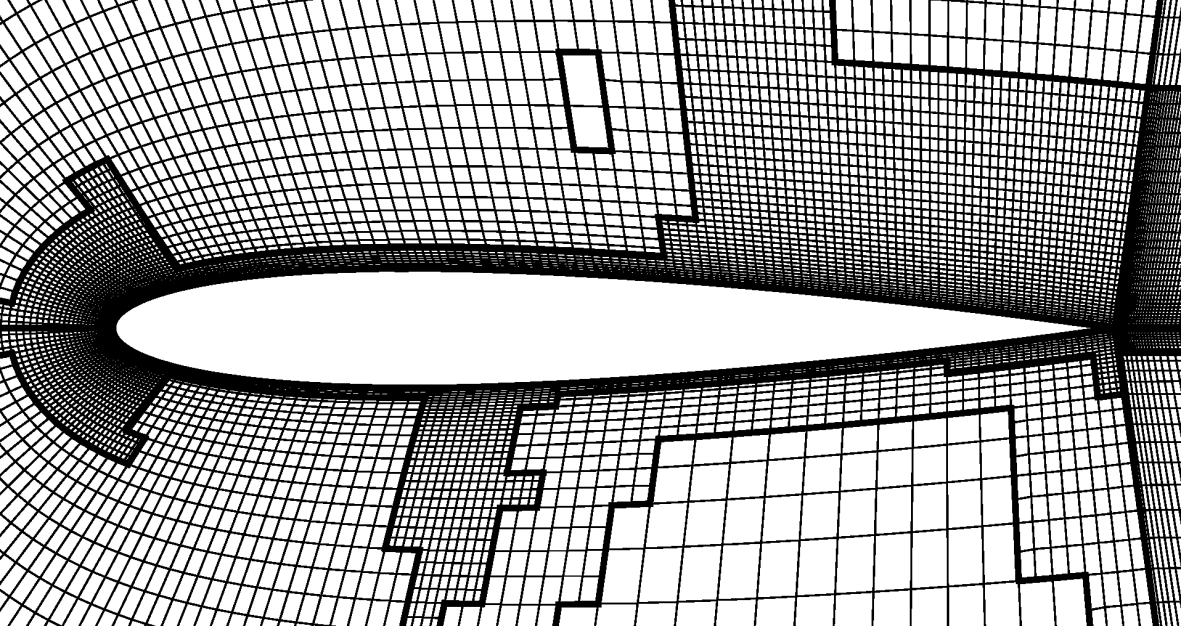
\includegraphics[width=0.46\textwidth]{profile}
\caption{A NACA0012 profile implemented in
QUADFLOW.}
\label{f:profile}
\end{figure}
%------------------------------------------------------------------------------------------
\end{frame}

\begin{frame}{Automatic Differentation}
After discretization of the differential equations solved in 
QUADFLOW and some reduction, it turns out that the
difficult part of solving the equation consists of computing the term involving the
Jacobian of the residual, i.e.,
\begin{equation*}
\frac{\partial \vek{R}(\vek{u}^n)}{\partial \vek{u}^n} \vek{z}.
\end{equation*}
Jacobian-vector products of this form are accurately and efficiently computed using
automatic differentiation.
\end{frame}

\begin{frame}{Automatic Differentation (2)}
Given a computer program evaluating some function $f: \R^n \rightarrow
\R^n$ at a point $\vek{x}_0\in \R^n$ and any user-chosen $n \times p$ seed matrix $S$,
the so-called forward mode of automatic differentiation generates a computer program to
evaluate not only $f(\vek{x}_0)$ but also the matrix-matrix product
$$
\left.\frac{\partial f(\vek{x})}{\partial \vek{x}}\right|_{\vek{x}=\vek{x}_0} \cdot S,
$$
where the $n \times n$ Jacobian
$$
J(\vek{x}_0) := \left.\frac{\partial f(\vek{x})}{\partial \vek{x}}\right|_{\vek{x}=\vek{x}_0}
$$
is evaluated at the same point $\vek{x}_0$ as the function $f$.
\end{frame}

\begin{frame}{Preconditioning}
In practice,
iterative solvers are rarely applied in a pure fashion, but involve some sort of
preconditioning.
$$J \vek{y}=\vek{b},\quad \vek{y} \in \R^n, \vek{b} \in \R^n, J \in \R^{n \times n}$$
Rather than solving the unpreconditioned system
 one is solving the preconditioned system
$$M^{-1} J \vek{y}= M^{-1}\vek{b},$$
A preconditioner somehow approximates the coefficient matrix,
$$M \approx J.$$
\end{frame}

\begin{frame}{Preconditioning (2)}
Common approaches to construct the preconditioner $M$ are based on accessing individual
nonzero entries $J(i,j)$ of the Jacobian:

\begin{itemize}
\item Diagonal Scaling 
\item LU factorization 
\item Incomplete LU factorization
\end{itemize}

\begin{alertblock}{Access to nonzero elements}
 In general, accessing an
individual nonzero entry via automatic differentiation is as efficient as accessing a
complete column or row. In practice, an access to some individual nonzero entry is
 expensive in terms of computing time.
\end{alertblock}
\end{frame}

\begin{frame}{Sparsification}
A sparsification of $J$, \sparsify{J}, selects a 
subset of all nonzero elements of $J$ and construct a
preconditioner based on these selected nonzero elements (required elements)
\begin{itemize}
\item Block Diagonal: the pattern of the required nonzero elements is
given by the pattern of all nonzero entries within these $k\times k$ blocks on the
diagonal. If the block size $k$ does not divide the matrix order $n$, we adapt the size
of the last diagonal block to some smaller value such that the sum of all block sizes
equals $n$.
\end{itemize}
\end{frame}

\begin{frame}{Sparsification (2)}
%------------------------------------------------------------------------------------------
\begin{figure}
\centering
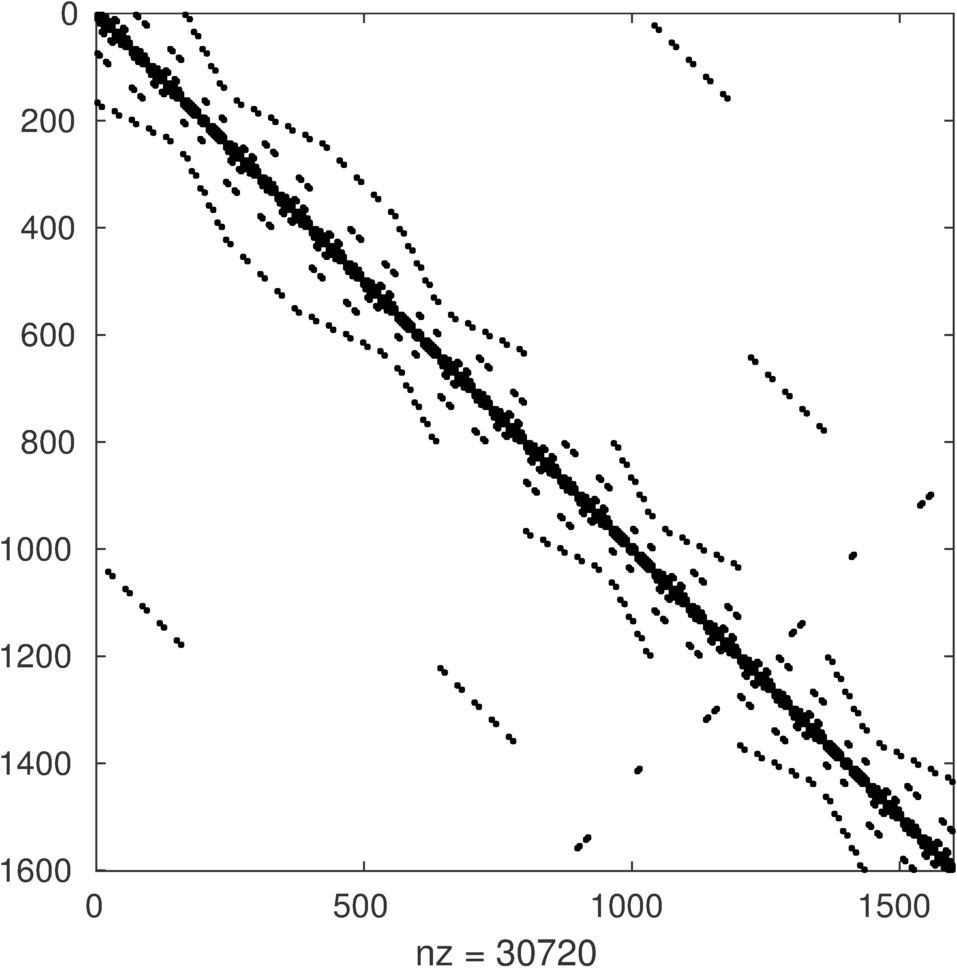
\includegraphics[width=0.42\textwidth]{quadflow}
\hfill
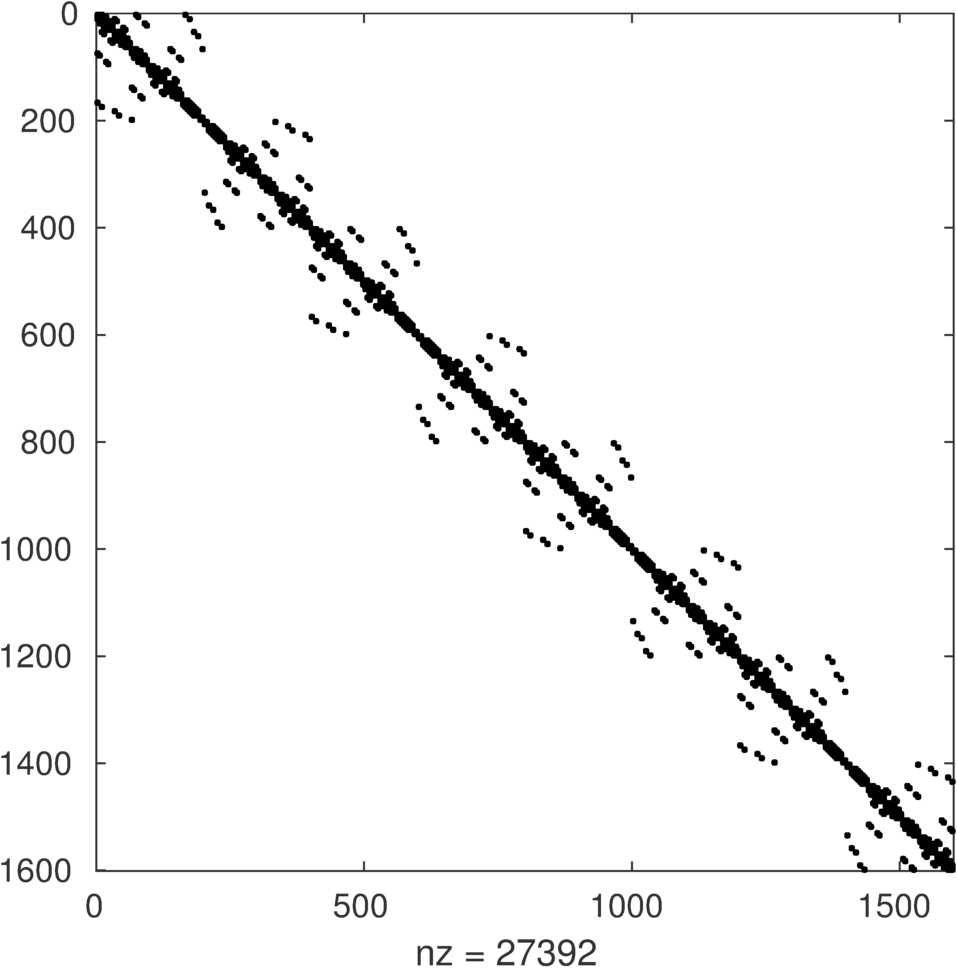
\includegraphics[width=0.42\textwidth]{block200}

\caption{Left: The nonzero pattern of the Jacobian $J$ with size $n=1,600$. 
Right: The pattern of the
sparsified Jacobian $\sparsify{J}$ illustrating the required elements for a block size of
$k=200$.}
\end{figure}
%------------------------------------------------------------------------------------------
\end{frame}
\begin{frame}{AD, Preconditioning, and Sparsification}
\begin{itemize}
  \item To perform a Jacobian-vector product $J \vek{z}$ with some vector \vek{z} in a
      iterative solver method, apply automatic differentiation with a seed matrix
      identical to that vector \vek{z}. 
  \item Choose a block size $k$ and apply the sparsification to get \sparsify{J} from
      the Jacobian~$J$. Assemble \sparsify{J} via automatic differentiation and store
      it explicitly.
  \item Construct a preconditioner $M$ from \sparsify{J} by performing an ILU(0)
      factorization on each block of~\sparsify{J}. 
\end{itemize}
\end{frame}

\begin{frame}{Full Jacobian Computation}

%------------------------------------------------------------------------------------------
\begin{figure}
\centering
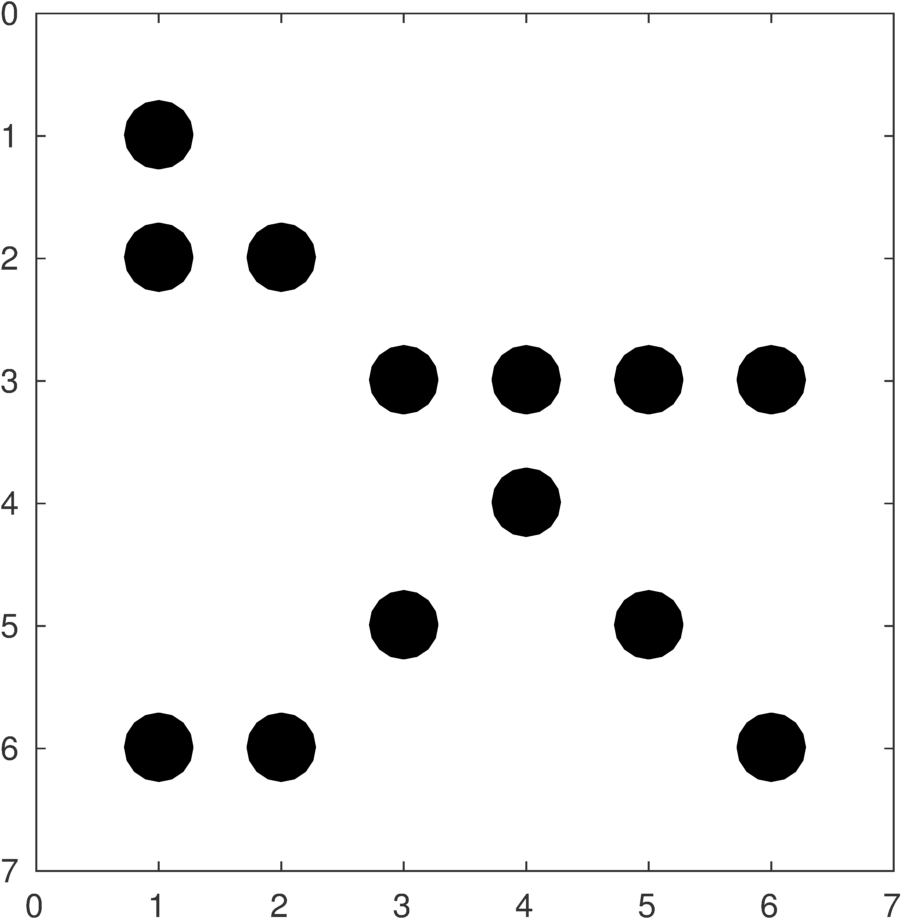
\includegraphics[height=0.27\textwidth]{small_jac}
\hfill
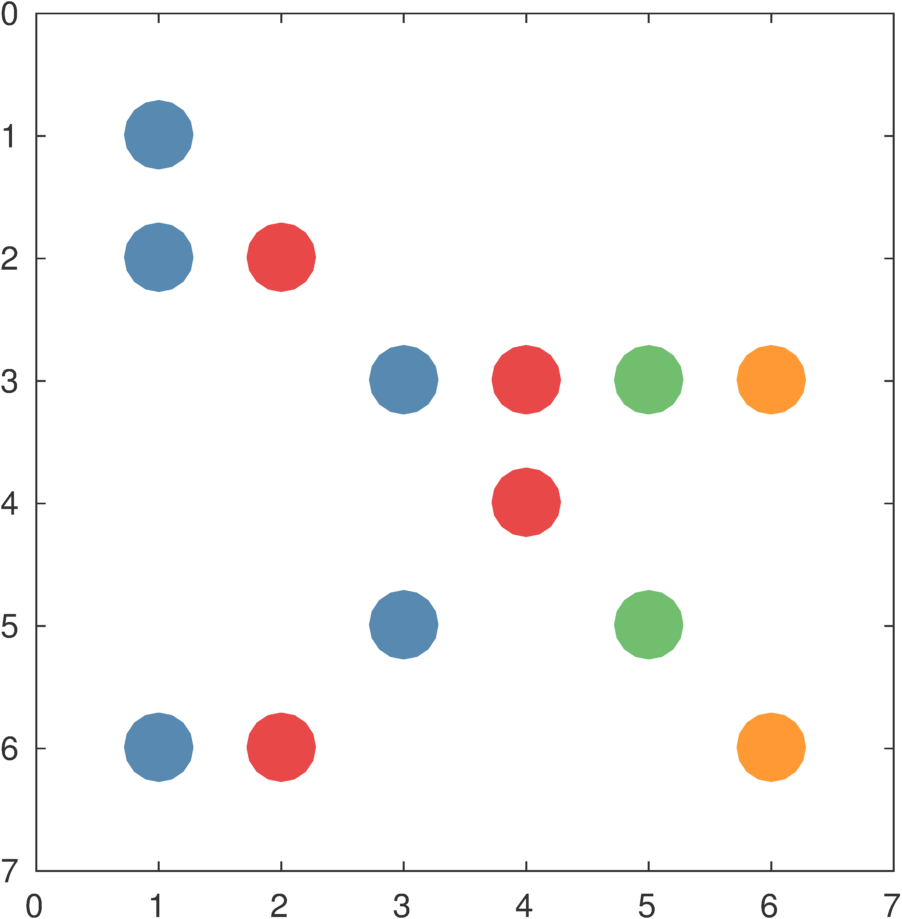
\includegraphics[height=0.27\textwidth]{full_color}
\hfill
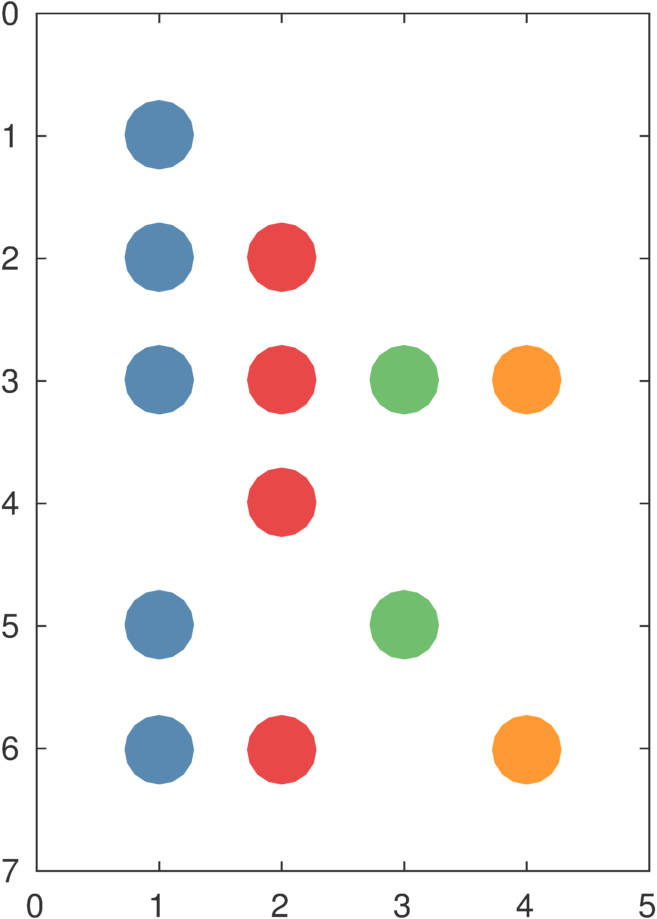
\includegraphics[height=0.27\textwidth]{full_color_compress}
\caption{Computation of all nonzero entries.
Left: The nonzeros are displayed in black. Middle: Each column is assigned a color.
Right: Columns with the same color are computed as linear combinations.}
%
\label{f:full}
\end{figure}
%------------------------------------------------------------------------------------------
\end{frame}
\begin{frame}{Partial Jacobian Computation}
%------------------------------------------------------------------------------------------
\begin{figure}[t]
\centering
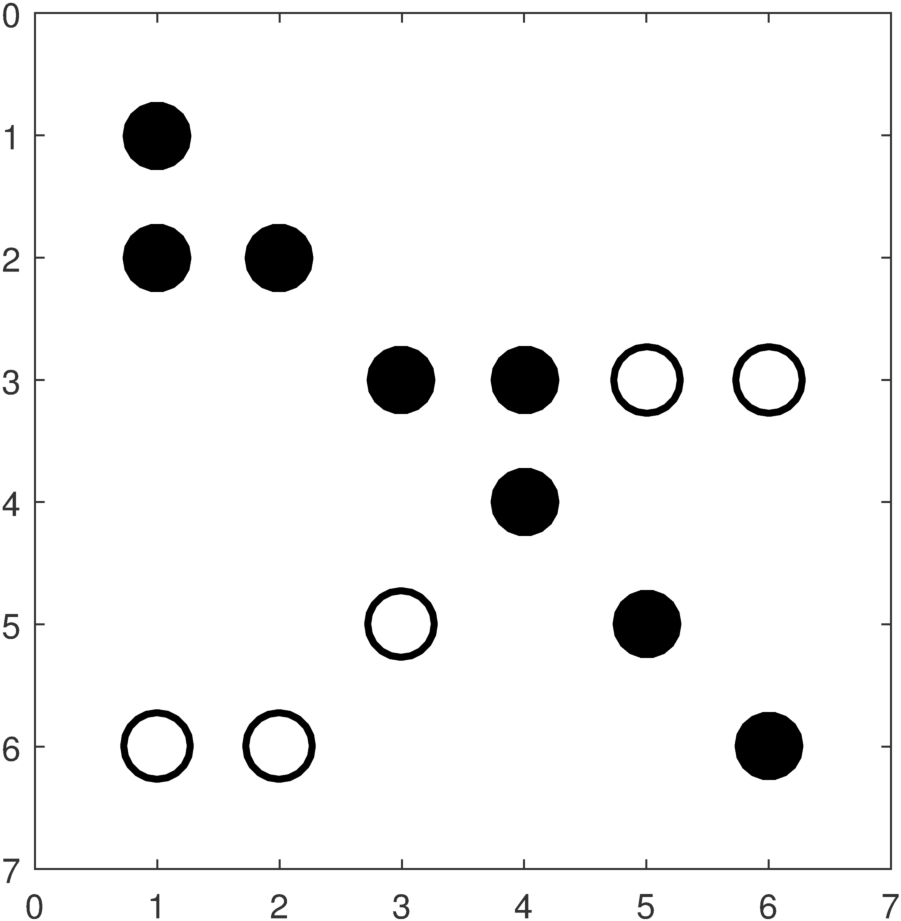
\includegraphics[height=0.27\textwidth]{partial_coloring_orig}
\hfill
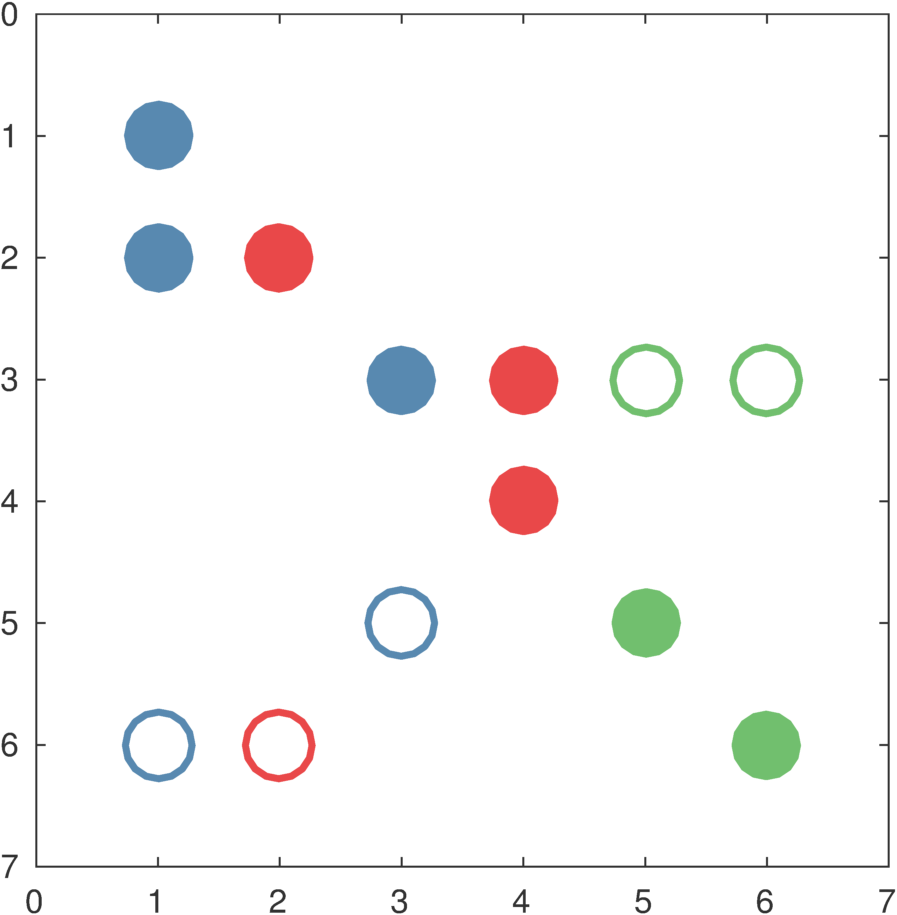
\includegraphics[height=0.27\textwidth]{partial_color}
\hfill
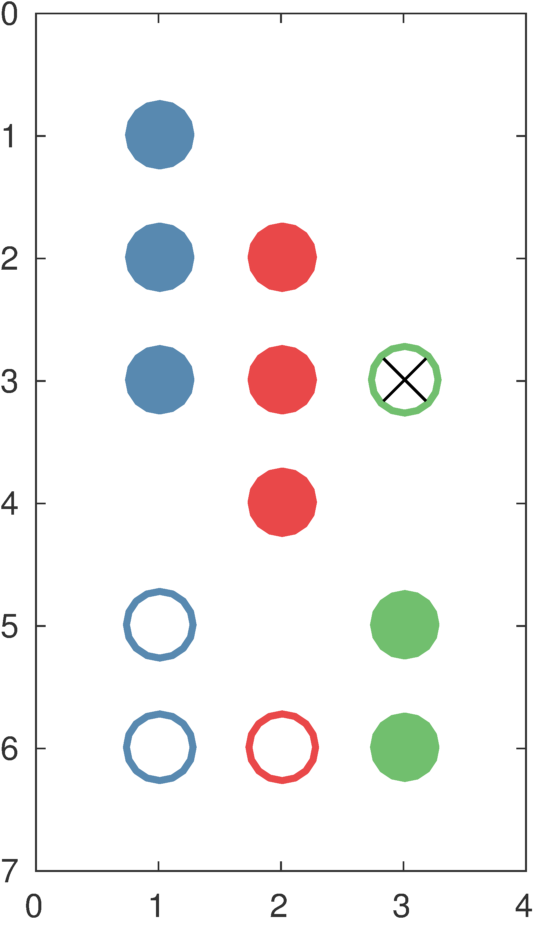
\includegraphics[height=0.27\textwidth]{partial_color_compress}
\caption{Computation of required nonzero entries.
Left: The nonzeros are subdivided into required elements (black disks) and
nonrequired elements (black circles). Middle: Each column is assigned a color.
Right: Columns with the same
color are computed as linear combinations.}
%
\label{f:partial}
\end{figure}
%------------------------------------------------------------------------------------------

\end{frame}

\begin{frame}{sparsify}
\begin{figure}
\centering
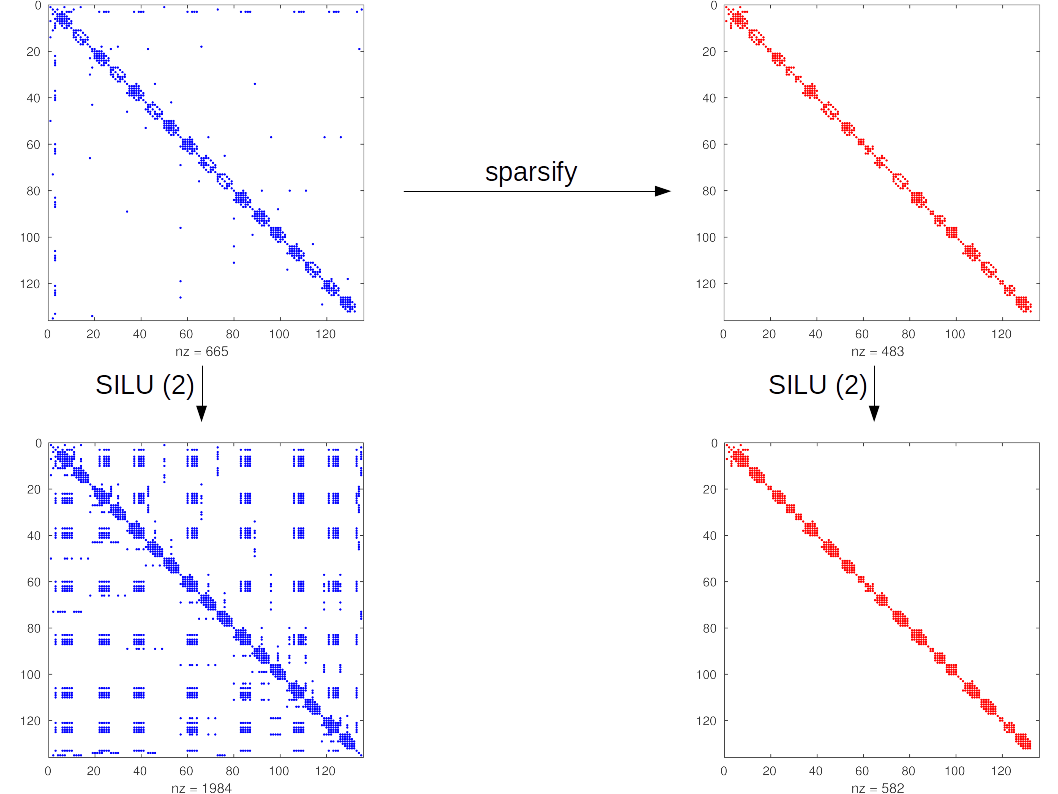
\includegraphics[width=0.8\textwidth]{sparsify}
\end{figure}
\end{frame}

\begin{frame}{Problem Formulation: Block Seed}
Let $J$ be a sparse $n \times n$ Jacobian matrix with known sparsity pattern and let
\sparsify{J} denote its sparsification using $k \times k$ blocks on the diagonal of $J$.
Find a binary $n \times p$ seed matrix~$S$ with a minimal number of columns, $p$, such
that all nonzero entries of \sparsify{J} also appear in the compressed matrix $J \cdot
S$.
\end{frame}

\begin{frame}{Combinatorial Model: Column Intersection Graph}
The column intersection graph $G = (V,E)$ associated with an $n \times n$ Jacobian $J$
consists of a set of vertices $V=\{v_1, v_2, \dots, v_n\}$ whose vertex $v_i$ represents
the $i$th column $J(:,i)$. Furthermore, there is an edge $(v_i,v_j)$ in the set of edges
$E$ if and only if the columns $J(:,i)$ and $J(:,j)$ represented by $v_i$ and $v_j$ have
a nonzero element in at least a same row position.
\end{frame}

\begin{frame}{Graph Coloring}
A coloring of $G$ is a mapping $\Phi : V \to {1, \dots, p}$ with the property
$\Phi(v_i)\neq \Phi(v_j)$ for $(v_i,v_j) \in E$.

\begin{alertblock}{Problem}
Find a coloring $\Phi$ of the column intersection graph $G$ with a minimal number of
colors.
\end{alertblock}
\end{frame}

\begin{frame}{structurally orthogonal}
A column $J(:,i)$ is structurally $\sparsifysymbol$-orthogonal to column $J(:,j)$ if and
only if there is no row position $\ell$ in which $J(\ell,i)$ and $J(\ell,j)$ are nonzero
elements and at least one of them belongs to the set of required element \sparsify{J}.
\end{frame}

\begin{frame}{$\sparsifysymbol$-Column Intersection Graph}
The $\sparsifysymbol$-column intersection graph $G_\sparsifysymbol =
(V,E_\sparsifysymbol)$ associated with a pair of $n \times n$ Jacobians $J$ and
\sparsify{J} consists of a set of vertices $V=\{v_1, v_2, \dots, v_n\}$ whose vertex
$v_i$ represents the $i$th column $J(:,i)$. Furthermore, there is an edge $(v_i,v_j)$ in
the set of edges $E_\sparsifysymbol$ if and only if the columns $J(:,i)$ and $J(:,j)$
represented by $v_i$ and $v_j$ are not structurally $\sparsifysymbol$-orthogonal.
\end{frame}

\begin{frame}{Minimum Block Coloring}
Find a coloring $\Phi$ of the $\sparsifysymbol$-column intersection graph
$G_\sparsifysymbol$ with a minimal number of colors.
\end{frame}

\begin{frame}{Experimental Results}

%------------------------------------------------------------------------------------------
\begin{figure}
\centering
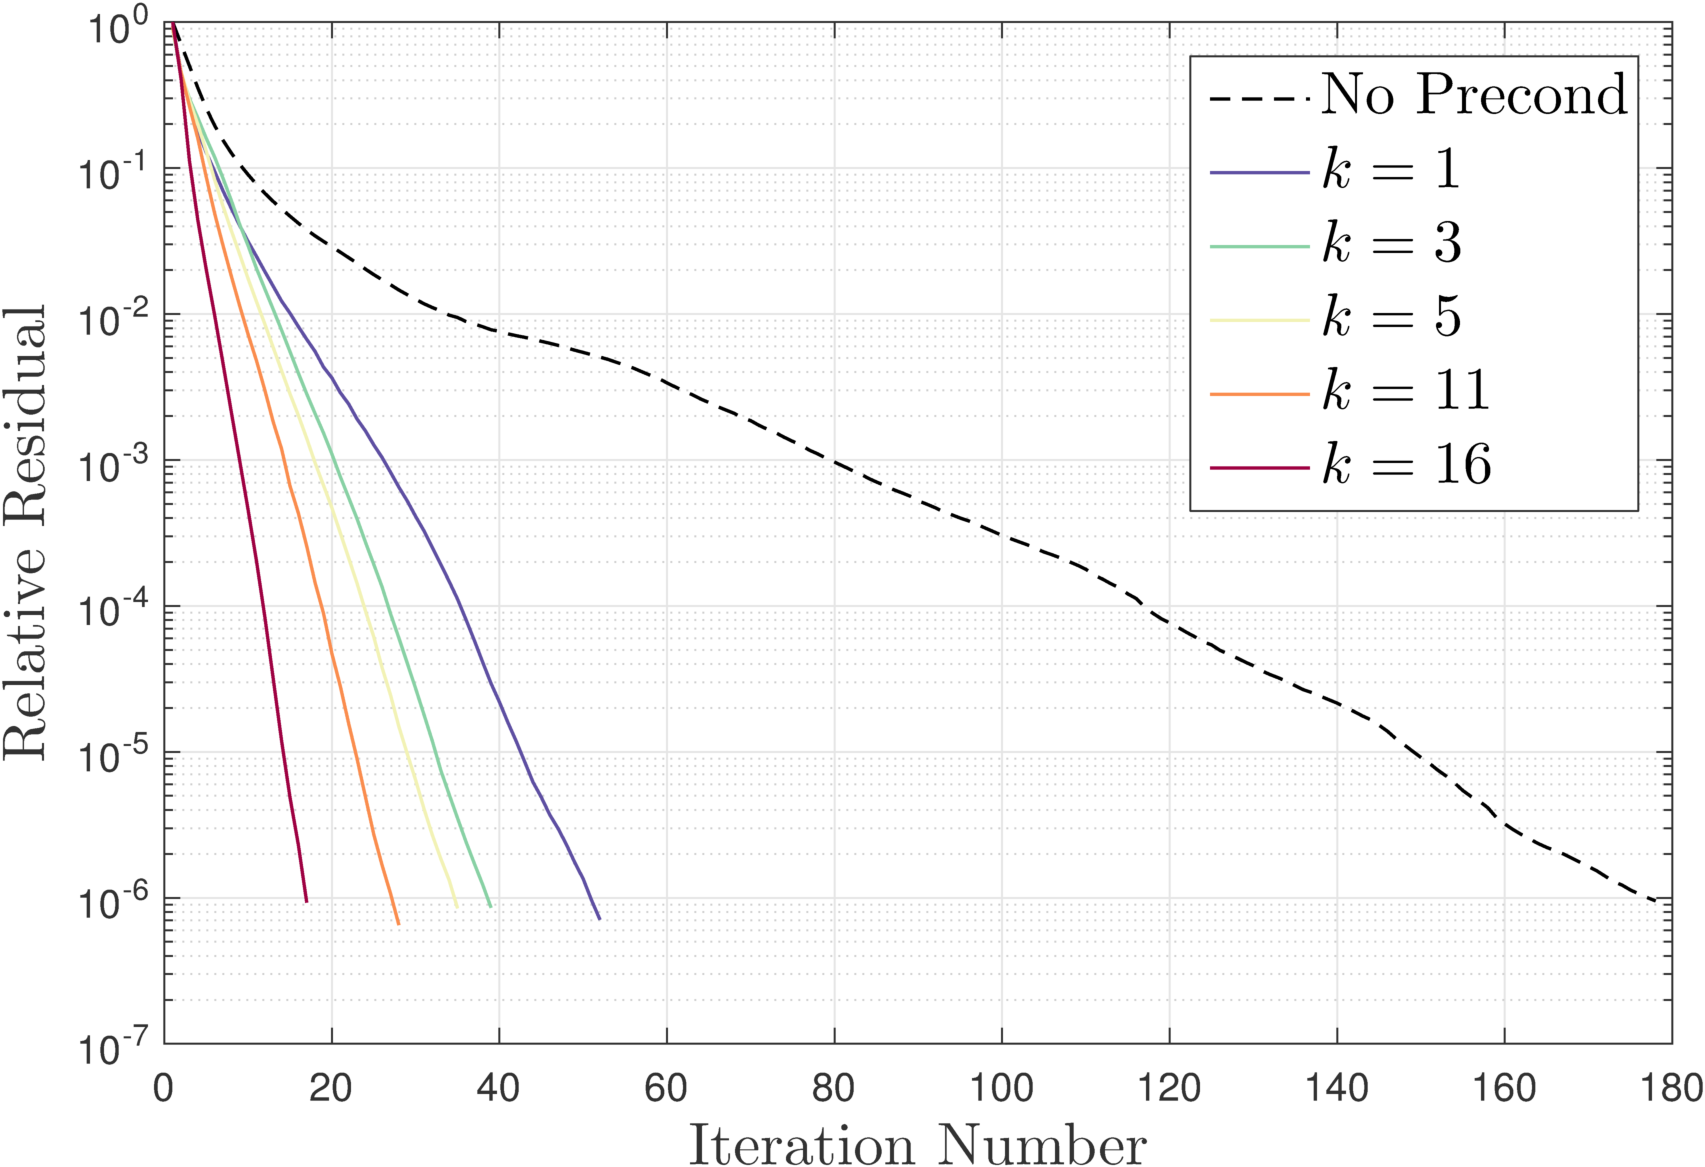
\includegraphics[width=0.48\textwidth]{convergence}
\caption{Convergence behavior varying the block size~$k$.}
\label{f:convergence}
\end{figure}
%------------------------------------------------------------------------------------------

\end{frame}

\begin{frame}{Required Elements vs Block sizes}
%------------------------------------------------------------------------------------------
\begin{figure}
\centering
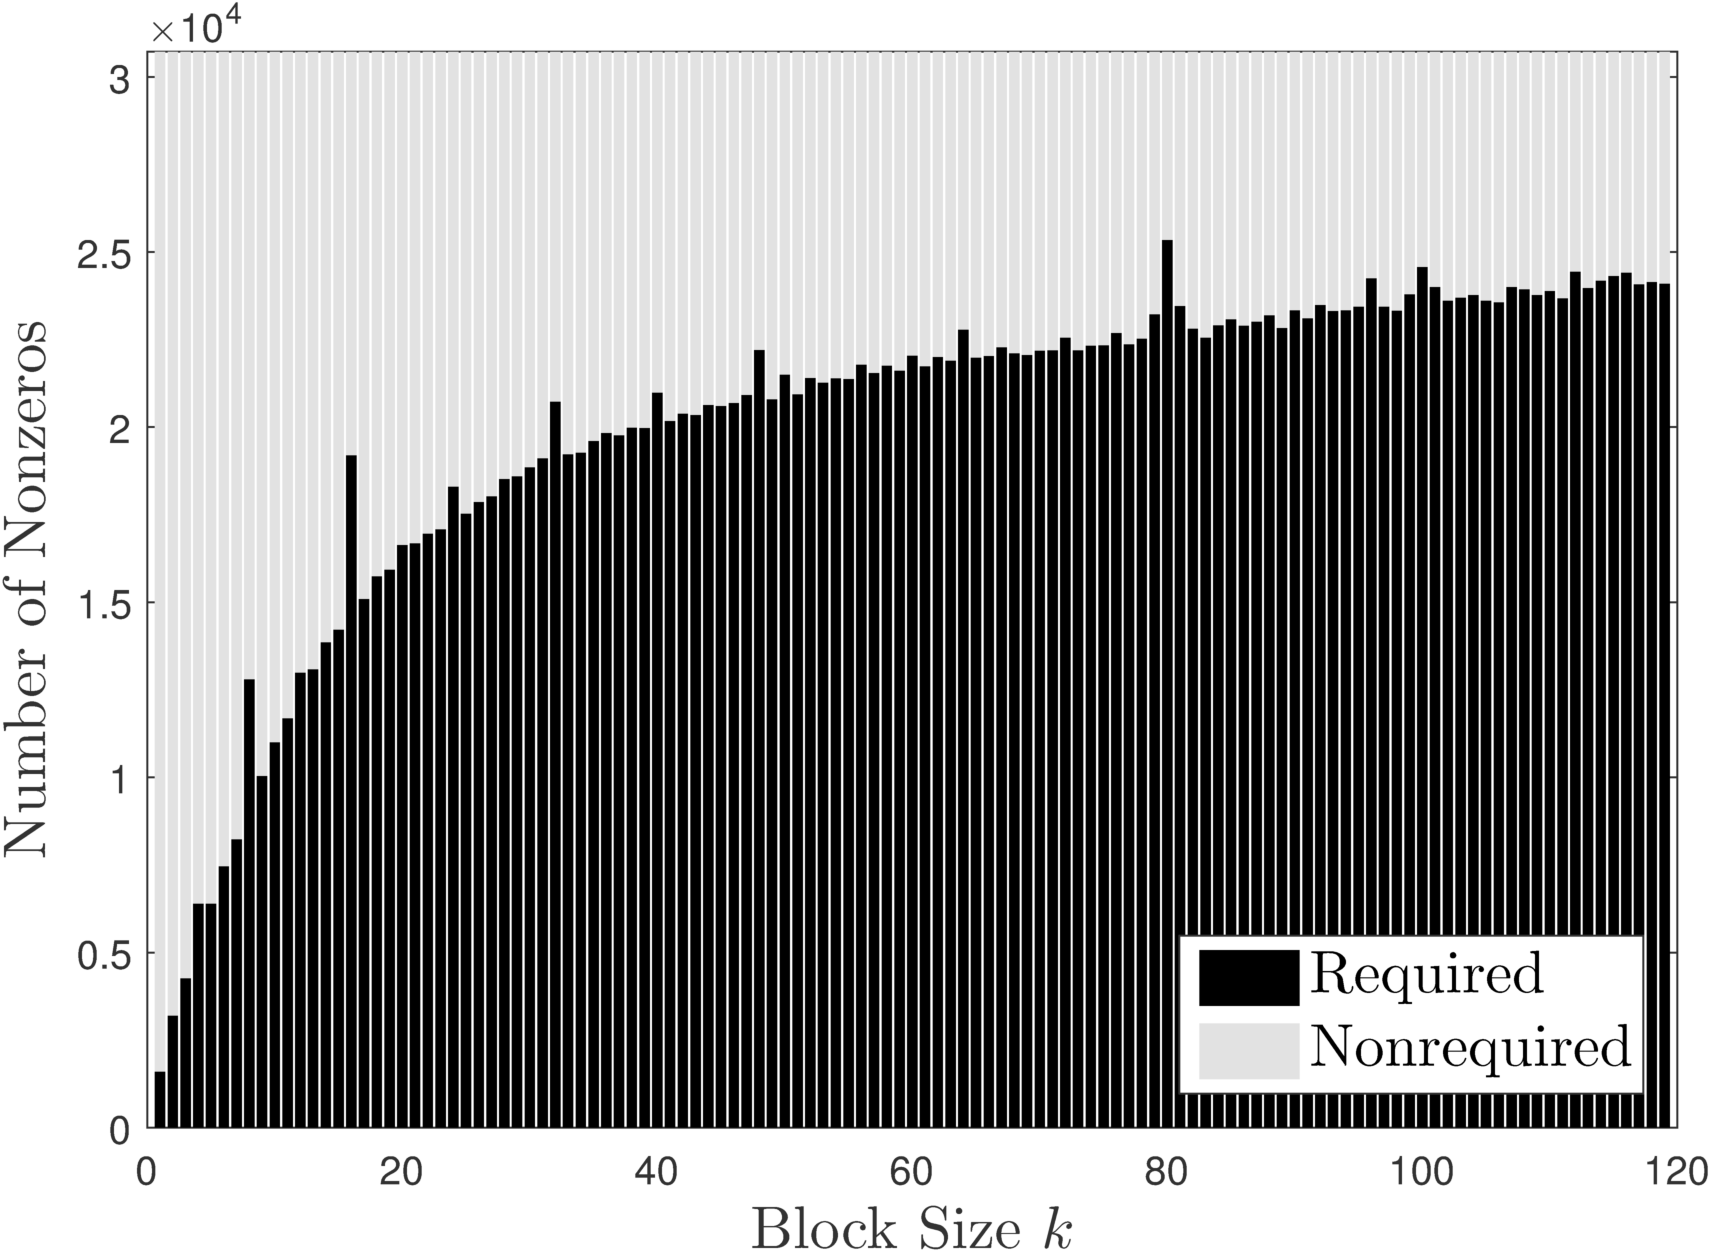
\includegraphics[width=0.45\textwidth]{nnz_bar_required_elements}
\caption{Number of required elements versus block size.}
\label{f:required_elements}
\end{figure}
%------------------------------------------------------------------------------------------
\end{frame}

\begin{frame}{Iterations vs Colors}
%------------------------------------------------------------------------------------------
\begin{figure}
\centering
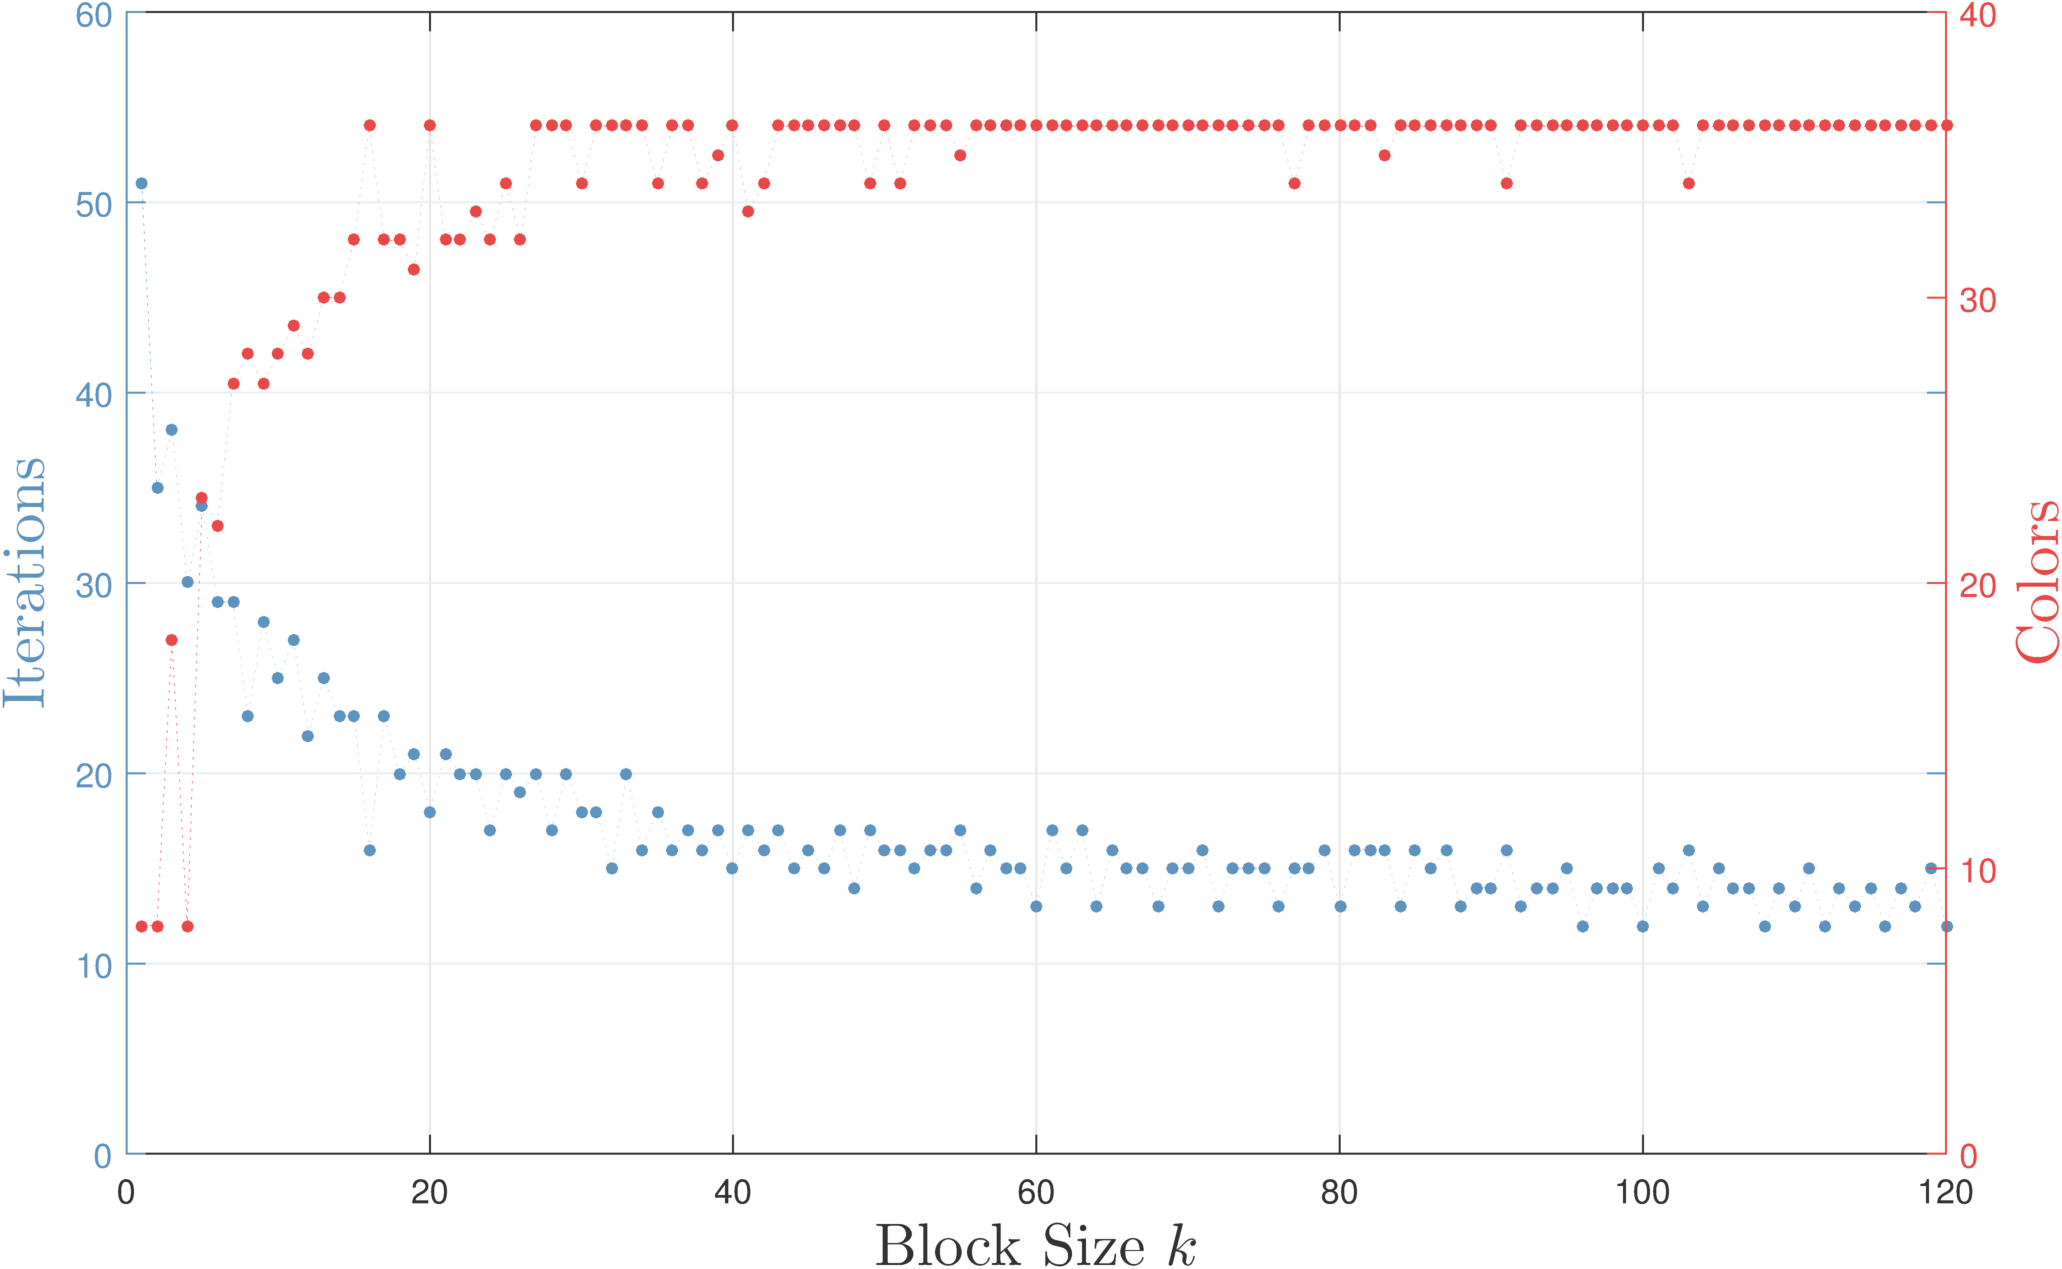
\includegraphics[width=0.75\textwidth]{iterations_colors}
\caption{The number of iterations needed to converge (given in blue) and the number of
colors needed by the coloring heuristic (given in red) both plotted versus the block size $k$.}
\end{figure}
%------------------------------------------------------------------------------------------
\end{frame}
\begin{frame}{Iterations vs Colors (2)}
\begin{figure}
\centering
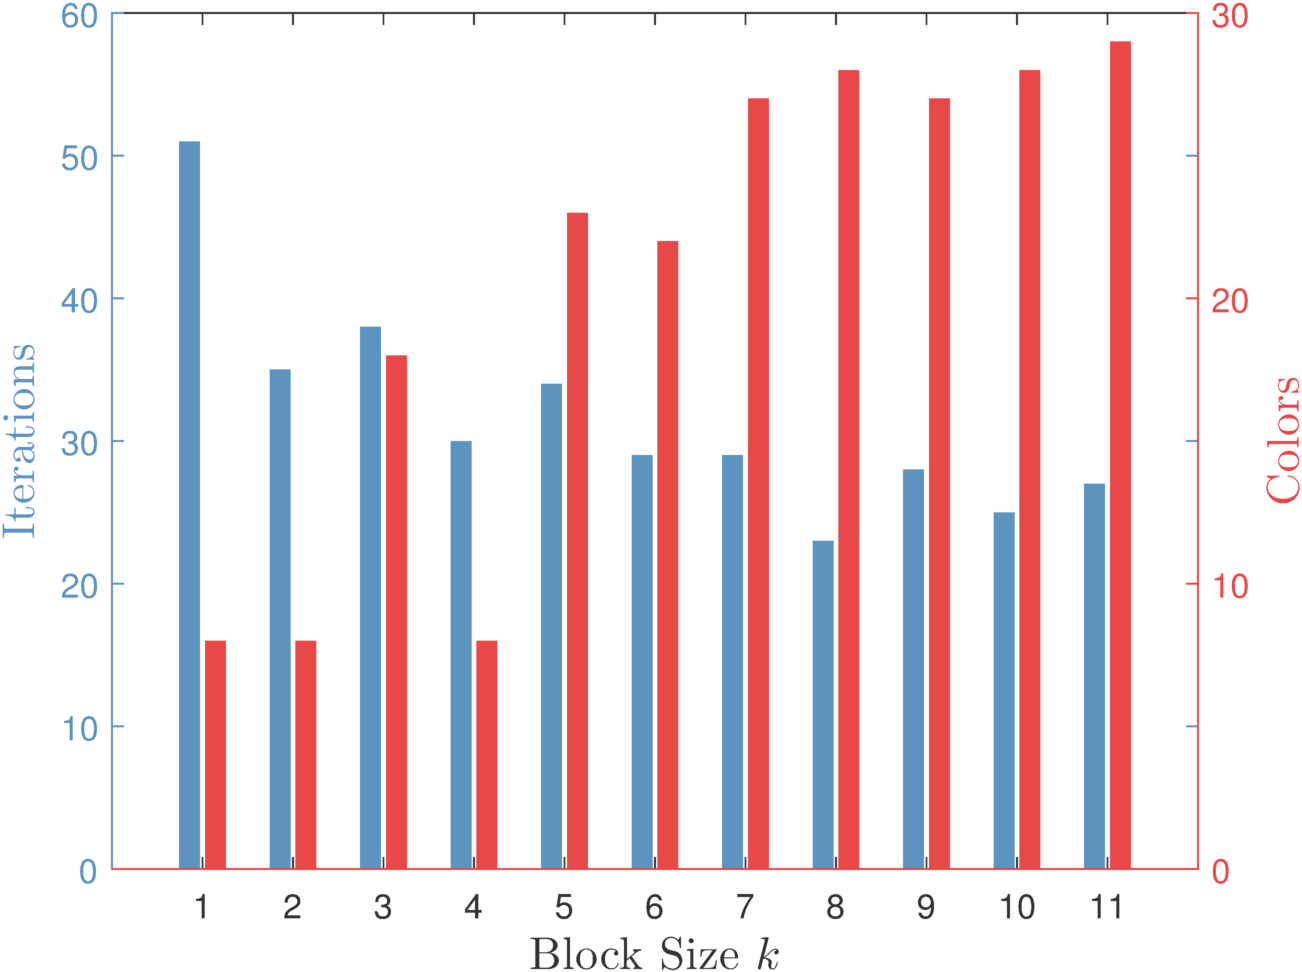
\includegraphics[width=0.44\textwidth]{zoom_iterations_colors}
\caption{Focus on $1 \leq k \leq 11$.}
\label{f:zoom_iterations_colors}
\end{figure}
\end{frame}

\begin{frame}{Timing results vs Block sizes}
%------------------------------------------------------------------------------------------
\begin{figure}
\centering
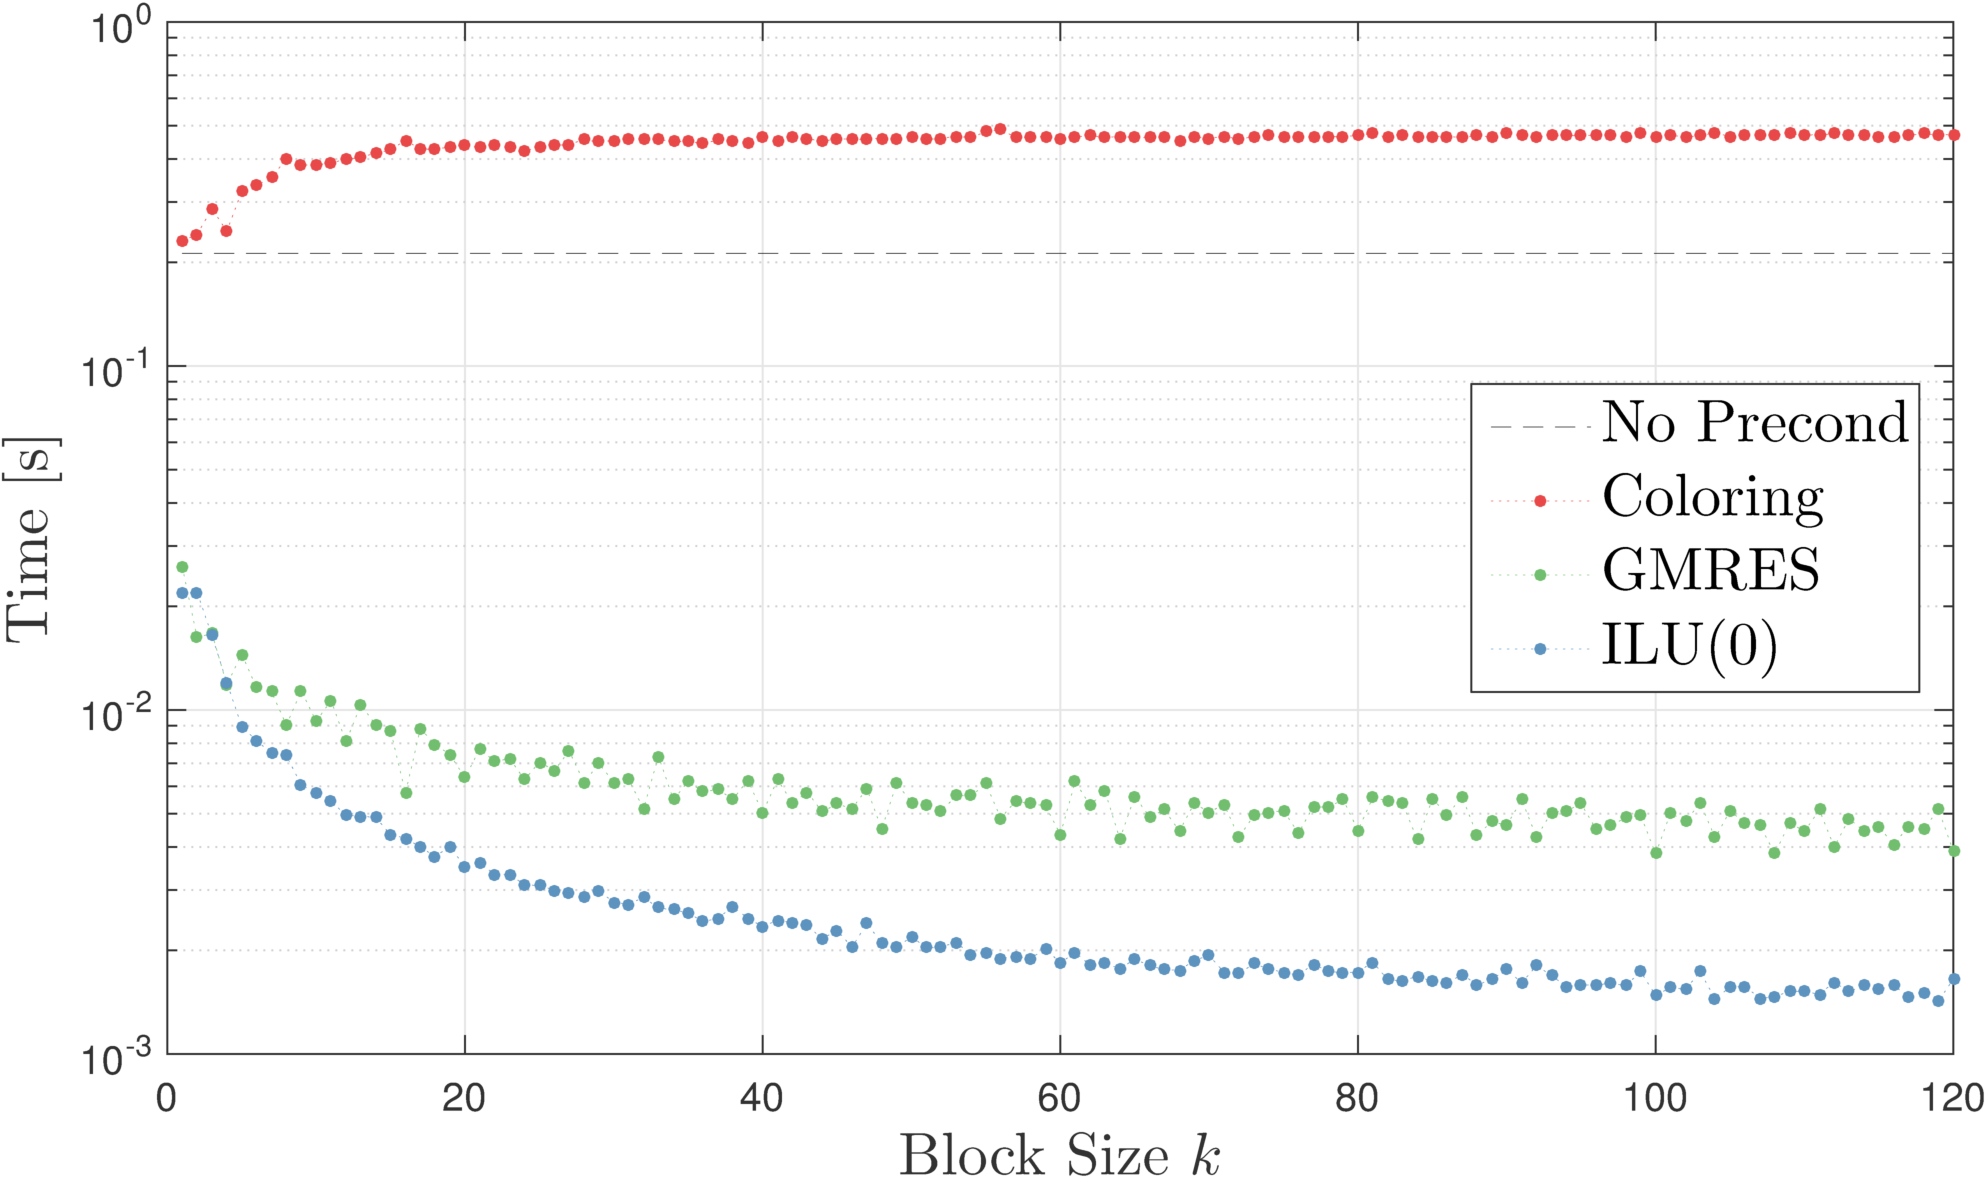
\includegraphics[width=0.8\textwidth]{timings}
\caption{The timing results in seconds of the different computational tasks plotted versus the block size $k$.}
\end{figure}
%------------------------------------------------------------------------------------------
\end{frame}
\begin{frame}{Conclusion}
\begin{itemize}
\item Automatic Differenation and Preconditioning together
\item Using partial Jacobian Computation
\item Modeling in graph language
\item Some experimental results
\end{itemize}
\end{frame}

\begin{frame}{Finish!}
\begin{center}
   \Huge \bf Thank you!
\end{center}
\end{frame}

\end{document}

